
\begin{ledgroupsized}[r]{120mm}
\footnotesize
\pstart
\noindent\textbf{Überlieferung:}
\pend
\end{ledgroupsized}
\begin{ledgroupsized}[r]{114mm}
\footnotesize
\pstart
\parindent -6mm
\makebox[6mm][l]{\textit{L}}%
Konzept:
LH~XXXV~9, 10~Bl.~5\textendash6. 
Ein Bogen~2\textsuperscript{o};
\href{\Scan{LH_35_09_10_005wz}}%
{Wasserzeichen} in Bl.~5.
Vier vorwiegend einspaltig beschriebene Seiten.
\pend
\end{ledgroupsized}
\selectlanguage{french}
\vspace{8mm}
\pstart
\centering
\href{\Scan{LH_35_09_10_005r}}%
{\lbrack5~r\textsuperscript{o}\rbrack}
\hfill
Demonstration\indexS{demonstration du principe de l'Equilibre}\indexS{demonstration analytique du Principe de l'Equilibre}
\edtext{analytique}{\lemma{}\Bfootnote{analytique \textit{erg.~L}}} 
du Principe de\indexS{principe de l'Equilibre}
\edlabel{35_09_10_005-006_1a}%
\edtext{}{\xxref{35_09_10_005-006_1a}{35_09_10_005-006_1b}\lemma{l'Equilibre}\Bfootnote{%
\textit{(1)}~\lbrack/\rbrack\ La demonstration d'Archimede dans son livre %
\textit{(2)}~Arc
\textit{(3)}~et qu'il y a un centre de gravité dans %
\textit{(a)}~tous les corps %
\textit{(b)}~toutes les figures \lbrack/\rbrack\
\textit{(4)}~Plusieurs~\textit{L}}}%
l'Equilibre
\hfill
\phantom{\lbrack5~r\textsuperscript{o}\rbrack}%
\linebreak
et qu'il y a un centre de gravité\indexS{centre de gravité} dans toutes les figures
\pend
\vspace{0.5\baselineskip}
\pstart
\noindent
Plusieurs\edlabel{35_09_10_005-006_1b} 
habiles Geometres\indexS{Geometres} 
\edtext{ont jugé}{%
\lemma{ont}%
\Bfootnote{%
\textit{(1)}~trouvé %
\textit{(2)}~jugé~\textit{L}}}
qu'il manque quelque chose à 
\edtext{la demonstration\indexS{demonstration d'Archimede} 
\indexN{\textls{Archimedes} 287\textendash212 v. Chr.}qu'Archimede\indexN{\textls{Archimedes} 287\textendash212 v. Chr.} 
a donné dans son livre \cite{01010}\textit{de aequiponderantibus}.}{\lemma{la demonstration \lbrack...\rbrack\ \textit{aequiponderantibus}}%
\Cfootnote{\indexN{\textls{Archimedes} 287\textendash212 v. Chr.}\textsc{Archimedes}, 
\cite{01010}\textit{De planorum aequilibris libri duo}, 
lib.~I, prop.~VI\textendash VII, S.\;152\textendash161.}} 
Il y en a d'autres qui la soûtiennent. Mais il n'est pas lieu icy d'entrer en cette discussion, et il sera plus à 
\edtext{propos de donner une nouvelle}{\lemma{propos}\Bfootnote{%
\textit{(1)}~de donner %
\textit{(2)}~de donner \bars{icy \textit{gestr.}} une %
\textit{(a)}~autre %
\textit{(b)}~nouvelle~\textit{L}}}
demonstration qui a des grands avantages, 
\edtext{sur celles que je me souviens}{\lemma{sur}\Bfootnote{%
\textit{(1)}~toutes les autres \bars{et celles \textit{erg.}} %
\textit{(2)}~celles
\textit{(3)}~celles que je me
\textit{(a)}~souvienne %
\textit{(b)}~souviens~\textit{L}}}
d'avoir veues. Car elle monstre 
\edtext{d'abord generalement}{\lemma{}\Bfootnote{%
d'abord
\bars{generalement \textit{erg.}}
que
\textit{(1)}~la distance \bars{des corps pesans \textit{erg.}} doit estre reciproque. Et elle le monstre sans distinction des proportions commensurables ou
\textit{(2)}~les 
\textit{(a)}~distances
\textit{(b)}~eloignements %
\textit{(aa)}~du centre de gravité de chaque corps et du point de l'equilibre, ou %
\textit{(aaa)}~de leur %
\textit{(bbb)}~du centre de gravité commun doivvent estre \bars{en raison \textit{erg.}} reciproque %
\textit{(aaaa)}~aux corps %
\textit{(bbbb)}~de celle des pesanteurs des corps, c'est à dire %
\textit{(aaaaa)}~à leurs %
\textit{(bbbbb)}~de leur grandeurs quand ils sont homogenes. 
\textit{(bb)}~des centres de gravité du centre
\textit{(aaa)}~de
\textit{(bbb)}~d'equilibre doivvent~\textit{L}}} 
estre en raison reciproque à celle des corps.\indexS{raison reciproque de deux corps} 
Soit que les corps soyent commensurables\indexS{commensurables} ou 
\edtext{non.\indexS{incommensurables} Au lieu}{\lemma{non.}\Bfootnote{%
\textit{(1)}~Au lieu %
\textit{(a)}~que les demonstrations %
\textit{(aa)}~que %
\textit{(bb)}~que j'ay %
\textit{(b)}~qu'on ne le prouve ordinairement, %
\textit{(aa)}~qu'on %
\textit{(bb)}~que dans le %
\textit{(2)}~Au lieu~\textit{L}}}
qu'on se contente ordinairement de le prouver 
\edtext{au commencement}{\lemma{}\Bfootnote{au commencement \textit{erg.~L}}}
dans les proportions commensurables\indexS{proportions commensurables} et de l'accommoder par apres aux incommensurables\indexS{proportions incommensurables} par une demonstration qui mene à l'impossible. 
\edtext{Mais ce qui est le principal, nostre}{\lemma{Mais}\Bfootnote{%
\textit{(1)}~le plus grand a %
\textit{(2)}~ce qui est le principal, %
\textit{(a)}~nostre %
\textit{(b)}~nostre~\textit{L}}}
demonstration est purement analytique;\indexS{demonstration analytique} 
c'est à dire elle monstre en même temps l'origine de l'invention.\indexS{origine de l'invention} 
Car il ne faut pas s'imaginer comme plusieurs qui sont entestés de l'Algebre,\indexS{Algebre} que l'analyse\indexS{analyse} n'est autre
\edtext{chose que la specieuse.\indexS{specieuse} 
L'analyse est \bracks{la methode}\indexS{methode analytique} 
de prendre la chose depuis sa source, de ne rien faire en tastonnant ny par rencontre, de ne rien supposer de dehors, ny de se servir d'aucune connoissance, à la quelle cette methode même ne mene\lbrack,\rbrack\ de faire voir par tout comment et pourquoy on s'est avisé de raisonner ainsi, et de prendre ce biais. En un mot d'aller par une voye dont on prevoit le succès. Car}{\lemma{chose que}\Bfootnote{%
\textit{(1)}~le calcul %
\textit{(a)}~d' %
\textit{(b)}~par 
\textit{(aa)}~symboles
\textit{(bb)}~lettres 
\textit{(2)}~la specieuse. 
\textit{(a)}~Toute la methode 
\textit{(aa)}~qui prend la chose depuis sa source, qui ne fait rien en tastonnant ny par rencontre, qui 
ne sert\lbrack\!\textit{!}\rbrack\ d'aucune connoissance 
\textit{(aaa)}~prise 
\textit{(aaaa)}~de
\textit{(bbbb)}~d'ailleurs, 
\textit{(bbb)}~,~à la quelle cette methode même ne mene,
et qui fait voir par tout comment \bars{et pourquoy \textit{erg.}} 
on \lbrack...\rbrack\ biais dont en s'est servi: est purement Analytique.
\textit{(bb)}~doi %
\textit{(b)}~La methode est tousjours analytique lors qu'on prend %
\textit{(c)}~L'analyse est \bars{la methode \textit{erg. Hrsg.}} de \lbrack...\rbrack\ ne mene
\bars{enfin \textit{erg.~u.~gestr.}}
de \lbrack...\rbrack\ biais.
\bars{En \lbrack...\rbrack\ voye
\textit{(1)}~qu'on prevoit d
\textit{(2)}~dont on prevoit le succès.~\textit{erg.}}
\textit{(aa)}~Par %
\textit{(bb)}~Dans l %
\textit{(cc)}~Car~\textit{L}}}
\edtext{icy par 
\edtext{exemple les corps}{\lemma{exemple}\Bfootnote{%
\textit{(1)}~quand %
\textit{(2)}~les corps~\textit{L}}}
pesans estans \textit{DEF}, et \textit{ACB}, la balance \textit{CE}, le point de l'equilibre\indexS{point de l'equilibre} \textit{G}. quand on prend \textit{G} en sorte que \textit{CG}, et \textit{EG} sont comme \textit{DEF}, \textit{ACB},}{%
\lemma{icy \bracks{...} \textit{DEF}, \textit{ACB}}%
\Cfootnote{Dem Text liegt das Diagramm \bracks{\textit{Fig.~1}} von N.\;\ref{41134} (S.~\pageref{Fig:35_09_10_001-002_fig-1}) zugrunde, das Leibniz am Ende des vorliegenden Konzepts (auf Bl.~6~v\textsuperscript{o}, hier S.~\pageref{Fig:35_09_10_005-006_fig-1}) mithilfe von Blindlinien und punktueller Perforierung des Papiers sehr genau nachgezeichnet hat.}}
pour prouver par là que \textit{G} est le point de l'equilibre,\indexS{point de l'equilibre} 
la demonstration peut estre bonne, mais la methode n'est pas telle qu'on la peut souhaiter,
\href{\Scan{LH_35_09_10_005v}}%
{\lbrack5~v\textsuperscript{o}\rbrack}  car comment est on allé s'aviser de diviser \textit{EC} 
\edtext{par le point \textit{G}}{\lemma{}\Bfootnote{par le point \textit{G} \textit{erg.~L}}} 
en raison reciproque des corps: si ce n'est peut estre parce qu'on sçavoit déja d'ailleurs que cela devoit reussir.
\edtext{Mais la veritable analyse\indexS{analyse}}{%
\lemma{Mais}%
\Bfootnote{%
\textit{(1)}~l'analyse
\textit{(2)}~la veritable analyse~\textit{L}}}
nous mene insensiblement à cette 
\edtext{division, si même}{\lemma{division,}\Bfootnote{%
\textit{(1)}~et sans %
\textit{(2)}~si même~\textit{L}}}
on n'en avoit pas entendu parler 
\edtext{auparavant. C'est}{%
\lemma{auparavant.}%
\Bfootnote{%
\textit{(1)}~J'ay jugé à propos de m'etendre la dessus
\textit{(2)}~C'est~\textit{L}}}
pourquoy il y a des demonstrations ou constructions qu'on a trouvées par la specieuse,\indexS{specieuse} mais 
\edtext{qui ne sont}{%
\lemma{qui ne}%
\Bfootnote{%
\textit{(1)}~laissent 
\textit{(2)}~sont~\textit{L}}}
pas pour cela analytiques.
\pend
\pstart 
J'ay jugé à propos de m'etendre la 
\edtext{dessus, parce que ces}{%
\lemma{dessus,}%
\Bfootnote{%
\textit{(1)}~à fin de
\textit{(2)}~parce que
\textit{(a)}~s
\textit{(b)}~ces~\textit{L}}}
reflexions sont
de consequence pour l'avancement de l'art d'inventer.\indexS{art d'inventer} Pour venir à la demonstration, 
\edtext{voicy comme}{%
\lemma{voicy}%
\Bfootnote{%
\textit{(1)}~comme j'ay fait pour la trouver. Soit la balance 
\textit{(2)}~comme~\textit{L}}}
j'y suis arrivé.
\pend
\pstart 
Soit la balance\indexS{balance} 
\edtext{\textit{EC} qu'on considere comme sans poids\lbrack,\rbrack\ les centres\indexS{centre de gravité} de gravit\lbrack é\rbrack\ des}{%
\lemma{\textit{EC}}%
\Bfootnote{%
\textit{(1)}~,~les corps
\textit{(2)}~\bars{qu'on considere comme sans poids \textit{erg.}} les centres de 
\bars{gravités \textit{ändert Hrsg.}} des~\textit{L}}}
corps attachés à la balance, \textit{C.E.} et les corps homogenes, et en raison donnée de \textit{DF} à \textit{AB}. Il s'agit de trouver le 
\edtext{point de l'equilibre,\indexS{point de l'equilibre} 
en sorte que la balance\indexS{balance} 
estant soutenue en \textit{G}}{\lemma{point}\Bfootnote{%
\textit{(1)}~\textit{G} %
\textit{(2)}~du soûtien, sçavoir \textit{G} %
\textit{(a)}~c'est à dire on la %
\textit{(b)}~tel que %
\textit{(3)}~de \lbrack...\rbrack\ en \textit{G}~\textit{L}}}
les corps \textit{C}, \textit{E} demeurent en 
\edtext{equilibre. Or}{\lemma{equilibre.}\Bfootnote{%
\textit{(1)}~Pour %
\textit{(2)}~Or~\textit{L}}}
l'on peut considerer toute la pesanteur des corps\indexS{pesanteur des corps considerée comme ramassée dans son centre} comme ramassée dans leurs centres de gravité\indexS{centre de gravité} \textit{C} et \textit{E}. Mais il est visible qu'on trouve plus de matiere de raisonner, quand on les 
\edtext{suppose etendus}{\lemma{suppose}\Bfootnote{%
\textit{(1)}~étendues %
\textit{(2)}~étendus~\textit{L}}}
par ce qu'ainsi on peut examiner chaque partie 
\edtext{à part. Or quoyqu'il importe}{\lemma{à part.}\Bfootnote{%
\textit{(1)}~Mais d %
\textit{(2)}~Or quoyqu'\bars{il \textit{erg.}} importe~\textit{L}}}
point à la 
\edtext{necessité de la}{\lemma{}\Bfootnote{necessité de la \textit{erg.~L}}}
demonstration quelle figure\indexS{figure du corps} on donne à ces corps, il peut neantmois importer 
\edtext{beaucoup à la commodité de}{\lemma{beaucoup}\Bfootnote{%
\textit{(1)}~à %
\textit{(2)}~à la commodité de~\textit{L}}}
l'invention. Et comme nous avons dit que ces corps entre eux sont 
\edtext{en raison}{%
\lemma{en}%
\Bfootnote{%
\textit{(1)}~raisons
\textit{(2)}~raison~\textit{L}}}
des droites \textit{DF}, et \textit{AB} 
\edtext{qui est la maniere la plus simple d'exprimer une raison.}{\lemma{}\Bfootnote{qui \lbrack...\rbrack\  raison \textit{erg.~L}}}
Supposons 
\edtext{donc}{\lemma{}\Bfootnote{donc \textit{erg.~L}}}
ces deux corps etendus comme ces lignes, c'est à dire supposons que ces sont deux 
\edtext{cylindres suspendus de la balance chacun par le point de son milieu\lbrack,\rbrack\ qui}{\lemma{cylindres}\Bfootnote{%
\textit{(1)}~egalement %
\bars{\textit{(1)}~attachés à %
\textit{(2)}~suspendus de la balance \bars{chacun \textit{erg.}} par le point %
\textit{(a)}~du milieu %
\textit{(b)}~de 
\textit{(aa)}~leur
\textit{(bb)}~son milieu \textit{erg.}}
qui~\textit{L}}}
ont la même epaisseur mais dont les longeurs
sont les droites \textit{DF}. et \textit{AB}. Car ainsi nous pourrons considerer ces corps, comme si ce n'estoient que des lignes 
\edtext{droites, puisque}{\lemma{droites,}\Bfootnote{%
\textit{(1)}~car %
\textit{(2)}~puisque~\textit{L}}}
l'epaisseur 
\edtext{estant la même de}{\lemma{estant}\Bfootnote{%
\textit{(1)}~de %
\textit{(2)}~la même de~\textit{L}}}
part et d'autre, ne change rien au 
\edlabel{35_09_10_005-006_3a}%
\edtext{}{\xxref{35_09_10_005-006_3a}{35_09_10_005-006_3b}\lemma{raisonnement.}\Bfootnote{%
\textit{(1)}~La situation %
\textit{(2)}~\href{\Scan{LH_35_09_10_006r}}%
{\lbrack6~r\textsuperscript{o}\rbrack} La %
\textit{(3)}~La %
\textit{(a)}~situation plus %
\textit{(b)}~situation plus simple et \bars{la \textit{gestr.}} plus~\textit{L}}}%
raisonnement.
\pend 
\pstart 
\href{\Scan{LH_35_09_10_006r}}%
{\lbrack6~r\textsuperscript{o}\rbrack} La situation plus simple et plus\edlabel{35_09_10_005-006_3b} 
naturelle de ces 
\edtext{corps \textit{DEF}. \textit{ACB}}{\lemma{corps}\Bfootnote{%
\textit{(1)}~entre eux %
\textit{(2)}~\textit{DF}. \textit{AB} %
\textit{(3)}~\textit{DEF}. \textit{ACB}~\textit{L}}}
entre eux et à l'egard de la balance est quand ils sont paralleles entre eux et perpendiculaires à la 
\edtext{balance. Par}{\lemma{balance.}\Bfootnote{%
\textit{(1)}~Mais cette situati %
\textit{(2)}~Par~\textit{L}}}
le point cherché \textit{G} menons \textit{PGQ} axe de l'equilibre\indexS{axe de l'equilibre} soutenant la
\edtext{\textit{CE}}{\lemma{}\Bfootnote{\textit{CE} \textit{erg.~L}}} 
\edtext{balance \textit{CE} en \textit{G} et}{\lemma{balance}\Bfootnote{%
\bars{\textit{CE} \textit{erg.}} en \textit{G}
\textit{(1)}~et parallele aux %
\textit{(2)}~per %
\textit{(3)}~perpendiculaire %
\textit{(4)}~et~\textit{L}}}
quoyque l'angle \textit{PGE} et \textit{PGC} puisse estre quelconque posons le droit; car c'est le plus simple. Mais comme nous ne voyons encor point de jour, pour découvrir le point \textit{G}. il faut que nous nous servions encor d'autres suppositions aussi faisables que celles que nous avons faites. Or il est manifeste, 
\edtext{que les corps \textit{DEF}. \textit{ACB} peuvent estre tournés à}{\lemma{que}\Bfootnote{%
\textit{(1)}~nous n'avons
\textit{(2)}~les %
\textit{(a)}~corps %
\textit{(b)}~lignes %
\textit{(c)}~corps \textit{DEF}. \textit{ACB} peuvent estre tournés %
\textit{(aa)}~sur leur centres de gravi %
\textit{(bb)}~à~\textit{L}}}
l'entour de leur centres \textit{E}. \textit{C}, c'est à dire qu'ils peuvent faire à la balance tel angle que nous 
\edtext{voulons car}{\lemma{voulons}\Bfootnote{%
\textit{(1)}~par %
\textit{(2)}~car~\textit{L}}}
au lieu que l'angle \textit{ACE} est droit, il pourra estre oblique, comme l'on voit dans la situation (\textit{A})\textit{C}(\textit{B}). Car il est 
\edtext{manifeste que l'equilibre\indexS{equilibre}}{\lemma{manifeste}\Bfootnote{%
\textit{(1)}~que %
\textit{(2)}~que %
\textit{(a)}~rien %
\textit{(b)}~l'equilibre~\textit{L}}}
demeure tousjous le même. Mais de ces situations obliques il faut choisir la plus commode à nostre raisonnement. C'est à dire une telle qui fasse voir 
\edtext{à veue d'oeil}{\lemma{}\Bfootnote{à veue d'oeil \textit{erg.~L}}}
l'equilibre 
\edtext{des corps \textit{DF}. \textit{AB}}{\lemma{}\Bfootnote{des corps \textit{DF}. \textit{AB} \textit{erg.~L}}} 
à l'egard de l'axe \textit{PQ}. Mais comment le ferons nous? C'est à dire comment est il possible de voir à veue d'oeil que deux corps inégaux\indexS{corps inégaux en equilibre} sont en 
\edtext{equilibre? Nous y arriverons ainsi: de}{\lemma{equilibre?}\Bfootnote{%
\textit{(1)}~Je %
\textit{(a)}~respond %
\textit{(b)}~reponds qu'on le peut faire en faisant en sorte qu'une partie %
\textit{(aa)}~de l'un %
\textit{(bb)}~du %
\textit{(2)}~Cela %
\textit{(3)}~Nous y arriverons ainsi: %
\textit{(a)}~deux c %
\textit{(b)}~de~\textit{L}}}
deux corps inegaux l'un est plus grand que l'autre, et le plus grand est celuy qui a une partie égale à l'autre tout entiere, par 
\edtext{exemple \textit{ZB}}{\lemma{exemple}\Bfootnote{%
\textit{(1)}~\textit{Z}(\textit{B}) partie de \textit{AB} %
\textit{(2)}~\textit{ZB}~\textit{L}}}
partie de \textit{AB} egale à \textit{DF}. Donc si \textit{ZB} 
\edtext{et \textit{DF} avoient}{\lemma{et \textit{DF}}\Bfootnote{%
\textit{(1)}~estoient le %
\textit{(2)}~avoient~\textit{L}}}
leurs 
\edtext{centres ou points de milieu \indexS{point de milieu} \textit{E} et \textit{X}}{\lemma{centres}\Bfootnote{%
\textit{(1)}~\textit{E} et \textit{X} ou milieux %
\textit{(2)}~ou points de milieu \textit{E} et \textit{X}~\textit{L}}}
également distans de l'axe \textit{PQ}, c'est à dire que les perpendiculaires à l'axe \textit{EG}, et \textit{XY} fussent égales; il est  
\edtext{visible que \textit{DF}}{\lemma{visible que}\Bfootnote{%
\textit{(1)}~les %
\textit{(2)}~\textit{DF}~\textit{L}}}
et \textit{ZB} seroient en equilibre; et pour faire que tout soit en equilibre\indexS{equilibre} il faut que le reste de \textit{AB}; sçavoir \textit{AZ} fût aussi en 
\edtext{equilibre, c'est à dire}{\lemma{equilibre,}\Bfootnote{%
\textit{(1)}~ce qui %
\textit{(2)}~c'est à dire~\textit{L}}}
que son point de milieu \textit{R} soit dans l'axe \textit{PQ}.
\pend
\pstart 
\href{\Scan{LH_35_09_10_006v}}%
{\lbrack6~v\textsuperscript{o}\rbrack}
Voila donc 
\edtext{ce grand}{\lemma{ce}\Bfootnote{%
\textit{(1)}~probleme %
\textit{(2)}~grand~\textit{L}}}
probleme de Mechanique\indexS{grand probleme de mecanique} (trouver le point de l'equilibre,\indexS{point de l'equilibre} \textit{G}.) reduit aux termes de la pure Geometrie,\indexS{Geometrie pure} c'est à dire au probleme 
\edtext{suivant. La droite \textit{DEF} (dont le milieu est \textit{E}) et la droite \textit{EC}}{\lemma{suivant.}\Bfootnote{%
\textit{(1)}~Dans la droite, %
\textit{(2)}~Les droites \textit{DEF}. et \textit{EC} %
\textit{(3)}~La droite \textit{DEF}. \bars{(dont \lbrack...\rbrack\ droite \textit{erg.}}
\textit{EC}~\textit{L}}}
estant données de grandeur et de 
\edtext{position; mais la droite \textit{AB} de grandeur et}{\lemma{position;}\Bfootnote{%
\textit{(1)}~et %
\textit{(2)}~mais la droite 
\textit{(a)}~\textit{Ab}
\textit{(b)}~\textit{AB} de grandeur
\textit{(aa)}~en sorte q %
\textit{(bb)}~et~\textit{L}}}
son point de milieu\indexS{point de milieu} \textit{C} de 
\edtext{position: trouver}{\lemma{position:}\Bfootnote{%
\textit{(1)}~trouver \textit{PGQ} %
\textit{(2)}~trouver~\textit{L}}}
le point \textit{G} dans la droite \textit{EC}, et l'angle \textit{ACE} en sorte que menant \textit{PGQ} perpendiculaire à \textit{CGE} et 
\edlabel{35_09_10_005-006_2a}%
prenant \textit{BZ} égale à \textit{FD}, et \textit{BX} égale à \textit{FE}\lbrack,\rbrack\ soit \textit{XY} (perpendiculaire à \textit{PQ}) egale à 
\edtext{\textit{EG}, et que \textit{AB}}{\lemma{\textit{EG},}\Bfootnote{%
\textit{(1)}~et \textit{AZ} %
\textit{(2)}~et que 
\textit{(a)}~\textit{Ab}
\textit{(b)}~\textit{AB}~\textit{L}}}
rencontre \textit{PQ} en \textit{R} point de milieu de \textit{AZ}. Ce probleme de Geometrie est aisé à resoudre car à cause des triangles semblables \textit{RGC}, \textit{RYX}\lbrack,\rbrack\ \textit{GC} sera à \textit{YX} c'est à dire à \textit{GE} comme \textit{RC} à \textit{RX}. Or est il que \textit{RC} est égale à \textit{DE}, et \textit{RX} à \textit{AC}, donc \textit{GC} est à \textit{GE} comme \textit{DE} à \textit{AC}, c'est à dire comme \textit{DF} 
\edtext{à \textit{AB}. C'est}{\lemma{à \textit{AB}.}\Bfootnote{%
\textit{(1)}~C'est à dire en raison reciproque des %
\textit{(2)}~C'est~\textit{L}}}
à dire il se trouve que la raison des distances\indexS{raison des distances} \textit{GE}, et \textit{GC}, 
\edtext{est reciproque}{%
\lemma{est}%
\Bfootnote{%
\textit{(1)}~raison
\textit{(2)}~reciproque~\textit{L}}}
à celle des corps\indexS{raison de deux corps} \textit{E}, \textit{C}.
\pend
\pstart
Il reste seulement de prouver que \textit{RC} est egale à \textit{DE}, et \textit{RX} à \textit{AC}. 
Ce qui est aisé, car \textit{RC} est $AC-AR$, 
et 
\edtext{\textit{AR} est moitié de \textit{AZ} et \textit{AZ} est 
$AB-ZB$\lbrack,\rbrack\ ou 
$AB-DF$ et la moitié de \textit{AZ} ou 
\textit{AR} toute entiere, est $AC-DE$.}{%
\lemma{\textit{AR} est}\Bfootnote{%
\textit{(1)}~\textit{AZ} %
\textit{(2)}~dimidia \textit{AZ} %
\textit{(3)}~moitié de \textit{AZ} et \textit{AZ} est $AB-ZB$,
\textit{(a)}~seu $AB-DE$ donc \textit{RC} est $AC-AB$ ergo \bars{et \textit{streicht Hrsg.}} dimidia \textit{AZ} est $AC-DE$ donc \textit{AR} est $AC-DE$, vel tota \textit{AR} %
\textit{(b)}~vel %
\textit{(c)}~ou \lbrack...\rbrack\ entiere, est \bars{est \textit{streicht Hrsg.}} 
$AC-DE$~\textit{L}}}
\edtext{}{\lemma{}\Afootnote{\foreignlanguage{ngerman}{\textit{Am Rand}:}
\begin{tabular}{ccc}
\textit{CX} & \groesser & \textit{CV}\\
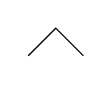
\begin{tikzpicture}\draw (-0.35,-0.65) -- (0.0,-0.3) -- (0.35,-0.65);\end{tikzpicture} & & 
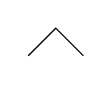
\begin{tikzpicture}\draw (-0.35,-0.65) -- (0.0,-0.3) -- (0.35,-0.65);\end{tikzpicture}\\
$CB-EF$ &  & $GE-CG$
\end{tabular}%
}} 
Donc \textit{RC} est $AC-AC+DE$. 
C'est à dire \textit{RC} est égale à \textit{DE}. Ce qui est le premier. 
D'où il est manifeste que \textit{RX} est égale à \textit{AC}, ou 
\textit{CB} ce qui estoit le second. Car de \textit{CB} ostons 
\textit{XB}, et adjoutons y \textit{RC}, et nous aurons 
\edtext{\textit{RX}, or}{%
\lemma{\textit{RX},}%
\Bfootnote{%
\textit{(1)}~et
\textit{(2)}~or~\textit{L}}}
nous avons autant 
\edtext{}{\lemma{}\Afootnote{\foreignlanguage{ngerman}{\textit{Am Rand}:} \textit{CV} difference entre \textit{GE} et \textit{CG}\lbrack,\rbrack\ \textit{CX} difference entre \textit{CB} et \textit{EF}.}} 
\edtext{adjouté qu'osté, puisque \textit{RC} est}{\lemma{adjouté}\Bfootnote{%
\textit{(1)}~que %
\textit{(2)}~qu'osté, puisque \textit{RC}
\textit{(a)}~est
\textit{(b)}~et
\textit{(c)}~est~\textit{L}}}
égale à \textit{XB} ou \textit{DE}. 
Donc la grandeur de \textit{RX} est la même que celle de \textit{CB}, c'est à dire 
\edlabel{35_09_10_005-006_4a}%
\edtext{}{%
\xxref{35_09_10_005-006_4a}{35_09_10_005-006_4b}%
\lemma{de \textit{AC}.}\Bfootnote{%
\lbrack/\rbrack\ 
\textit{(1)}~que %
\textit{(2)}~quand %
\textit{(3)}~Quand~\textit{L}}}%
de \textit{AC}.
\pend
\pstart
Quand\edlabel{35_09_10_005-006_4b}
le point \textit{G} est trouvé on n'a pas besoin de chercher l'angle \textit{ACE} mais si on le demande pour voir à l'oeil ce que nous avons demonstré  
\edtext{et pour donner la synthese\indexS{synthese} de nostre analyse\indexS{analyse}}{\lemma{}\Bfootnote{et pour donner la synthese de nostre analyse \textit{erg.~L}}} 
on peut faire ainsi: Du point \textit{G} soit prise \textit{GV} égale à \textit{GE} d'où il 
\edtext{soit abbaissée \textit{VX} parallele}{\lemma{soit}\Bfootnote{%
\textit{(1)}~\textit{VX} parallele à \textit{GQ} %
\textit{(2)}~abbaissée \textit{VX} %
\textit{(a)}~egale %
\textit{(b)}~parallele~\textit{L}}}
à \textit{GQ}. Du centre \textit{C}, 
\edtext{rayon \textit{CX} (c'est à dire $CB -BX$}{\lemma{rayon \textit{CX}~(}\Bfootnote{%
\textit{(1)}~c'est à dire $CB-LC$) %
\textit{(2)}~c'est à dire $CB - BX$~\textit{L}}}
ou $CB -EF$) soit decrit un 
\edtext{arc de cercle}{\lemma{arc}\Bfootnote{%
\textit{(1)}~coupant %
\textit{(2)}~de cercle~\textit{L}}}
coupant \textit{VX} 
\edtext{en \textit{X}. et en}{\lemma{en \textit{X}.}\Bfootnote{%
\textit{(1)}~en %
\textit{(2)}~et en~\textit{L}}}
même temps du centre 
\edtext{\textit{C}, et rayons}{\lemma{}\Bfootnote{\textit{C}, \bars{et \textit{erg.}} rayons~\textit{L}}}
\textit{CA}, \textit{CB}\bracks{,} soyent decrits les 
\edtext{arcs \textit{Aa} et \textit{Bb}.}{\lemma{arcs}\Bfootnote{%
\textit{(1)}~\textit{A}(\textit{A}) et \textit{B}(\textit{B}) %
\textit{(2)}~\textit{Aa} et \textit{Bb}.~\textit{L}}}
Continués la droite \textit{CX} de part et d'autre jusqu'à ce qu'elle rencontre ces arcs 
\edtext{en \textit{a} et \textit{b}}{\lemma{en}\Bfootnote{%
\textit{(1)}~(\textit{A}) et (\textit{B}) %
\textit{(2)}~\textit{a} et \textit{b}~\textit{L}}}
et nous 
\edtext{aurons l'inclination ou}{\lemma{aurons}\Bfootnote{%
\textit{(1)}~la %
\textit{(2)}~l'inclination ou~\textit{L}}}
situation 
\edtext{du corps \textit{AB}}{\lemma{}\Bfootnote{du corps \textit{AB} \textit{erg.~L}}} 
propre à nostre demonstration. Car il est visible que \textit{XY} est égale à \textit{VG} ou \textit{GE}, et que \textit{ZX}. \textit{XB}. \textit{DE}. \textit{EF} sont egales par la construction, donc \textit{ZB} et \textit{DF} sont en balance.\indexS{balance} Il est manifeste aussi et aisé à demonstrer par une synthese\indexS{synthese} opposée à l'analyse\indexS{analyse} de cydessus, que \textit{AR} est egale à \textit{RZ}, le point \textit{R} estant celuy où le corps \textit{AB}
\edtext{incliné comme}{\lemma{incliné}\Bfootnote{%
\textit{(1)}~comme nous venons de %
\textit{(2)}~comme~\textit{L}}}
nous avons dit, coupe l'axe \textit{PQ}. Donc \textit{AZ}
est aussi en equilibre, donc il n'y a rien qui puisse agir par sa pesanteur.%
\edlabel{35_09_10_005-006_2b} 
\edtext{Mais afin de ne rien laisser en arriere, adjoutons la synthese\indexS{synthese} dans la feuille suivante.}{%
\lemma{Mais \bracks{...} suivante}%
\Cfootnote{Gemeint ist wohl der Abschnitt von N.\;\ref{41134} ab \refpassage{35_09_10_001-002_8a}{35_09_10_001-002_8a} ("Voicy la synthese la plus commode qui on peut tirer de cette analyse.")}}
\pend 
\begin{edfigure}%
\includegraphics[scale=1]{%
gesamttex/edit_VIII-4/images/LH_35_09_10_005-006_d_006v.pdf}
\edcaption{%
\pagelabel{Fig:35_09_10_005-006_fig-1}%
\edtext{\lbrack\textit{Fig.~1, tlw. Blindzeichnung}\rbrack}{%
\lemma{\lbrack\textit{Fig.~1}\rbrack}%
\Cfootnote[nonum]{%
Bei der Anfertigung der Zeichnung hat Leibniz an dieser Stelle das Diagramm \bracks{\textit{Fig.~1}} von N.\;\ref{41134} (S.~\pageref{Fig:35_09_10_001-002_fig-1}) mithilfe von Blindlinien und punktueller Perforierung des Papiers sehr genau nachgezeichnet.
Leibniz hat zunächst die Punkte des gedrehten Körpers mit \textit{A}, \textit{B} bezeichnet und sie anschließend in \textit{a}, \textit{b} unbenannt. Diese Änderung hat er im Text auf \refpassage{35_09_10_005-006_2a}{35_09_10_005-006_2b} jedoch nicht berücksichtigt.
Ein gestrichener Entwurf zum Diagramm wird nicht wiedergegeben.}}}
\end{edfigure}
\selectlanguage{ngerman}
